% arara: indent: {overwrite: yes, trace: yes, files: [main.tex, domain.tex] }

\documentclass[a4paper,12pt,oneside,onecolumn]{book}
\usepackage{frontespizio}
\usepackage[italian]{babel}
\usepackage{ucs}
\usepackage[utf8x]{inputenc}
\usepackage{caption}
\usepackage{subcaption}
\captionsetup{compatibility=false}
\usepackage{graphicx}
\usepackage{mathtools}
\usepackage{amsmath}
\usepackage{hyperref}
\usepackage{color,soul}
\usepackage{multicol}
\usepackage{longtable}
\usepackage{enumitem}
\usepackage{titlesec}
\usepackage{algorithm}
\usepackage[noend]{algpseudocode}
\usepackage{listings}
\usepackage{rotating}
\usepackage[round,numbers]{natbib}
\setcitestyle{square}
\usepackage{moreverb}
\usepackage{mdframed}
\mdfsetup{frametitlealignment=\center, frametitlerule=true, leftmargin=-1.2cm, rightmargin=-2cm}
\usepackage{nameref}
\usepackage{array}
\newcolumntype{H}{>{\setbox0=\hbox\bgroup}c<{\egroup}@{}}
\usepackage{tabularx}
\usepackage{tabu}
\usepackage{ltxtable}
\usepackage{pdfpages}
\usepackage{floatpag}
\usepackage[strict]{changepage}
\usepackage{tabto}
\usepackage{adjustbox}
\usepackage{diagbox}
\usepackage{caption}
%\usepackage{minted}



\titleformat{\chapter}[hang]
{\normalfont\huge\bfseries}{\chaptertitlename\ \thechapter:}{0.3em}{}

\title{Crossroads Project}

\begin{document}
\begin{frontespizio}	
			
	\Preambolo{\renewcommand{\fronttitlefont}{%
		\fontsize{20}{24}\scshape}}
				
	\Universita{Bari}
	\Logo[1.5cm]{./images/logo}
	\Dipartimento{Informatica}
	\Corso[Laurea Magistrale]{Informatica}
	\Titoletto{Progetto di Intelligenza Artificiale}
	\Titolo{Incroci}
	\NCandidato{Esaminando}
	\Candidato[591275]{Giuseppe Rizzi}
	\NRelatore{Docente}{Docenti}
	\Relatore{Prof.~Floriana Esposito}
	\Relatore{Prof.~Nicola Di Mauro}
	\Piede{}
\end{frontespizio}
	    
%Ridefinizione di "for all" in "for each"
\renewcommand{\algorithmicforall}{\textbf{for each}}


\renewcommand{\labelitemiii}{$\circ$}

    
%Cambio l'intestazione "Algorithm" in "Algoritmo"
\floatname{algorithm}{Algoritmo}

%Numerazione delle pagine corretta
\pagestyle{plain}
\floatpagestyle{plain}
	
%Le tabelle larghe quanto la pagina
%	\setlength\LTleft{0pt}
%	\setlength\LTright{0pt}
%Da usare anche \begin{longtable}{@{\extracolsep{\fill}}| c | l |}
	
\tableofcontents
	
\newpage
\chapter{Introduzione}

Il presente documento mira a descrivere il progetto di Intelligenza Artificiale relativo alla costruzione di un sistema scritto in \emph{Prolog} per la risoluzione di incroci, tipici nei quiz degli esami per l'ottenimento della patente di guida. Il programma dovrà quindi essere in grado di restituire l'ordine di circolazione dei veicoli coinvolti dopo aver ottenuto in ingresso una descrizione dell'incrocio.

Per come si presentano veicoli, segnali e bracci all'interno di un incrocio, è intuitivo descrivere queste componenti tramite relazioni di oggetti, utilizzando un formalismo logico che, in questo caso, risulta molto più comodo rispetto ad un linguaggio imperativo. 

Il lavoro si svolgerà in diverse fasi, dallo studio del dominio alla creazione del software, fino al collaudo su esempi reali.

\clearpage
\chapter{Studio del dominio}

\section{Intersezioni}
Si definisce intersezione stradale l'area individuata da tre o più bracci (o tronchi) stradali che convergono in uno stesso punto, nonché dai dispositivi e dagli apprestamenti atti a consentire ed agevolare le manovre per il passaggio da un tronco all'altro.
Le intersezioni, qualunque sia la loro localizzazione territoriale, costituiscono punti critici del sistema viario per effetto delle interferenze che in esse si instaurano tra le diverse correnti di traffico.

È possibile suddividerle per categorie generali con riferimento all'ambito territoriale ed alla tipologia dell'incrocio. Relativamente all'ambito territoriale si hanno quindi intersezioni extraurbane ed intersezioni urbane. Per le prime elementi caratterizzanti risultano la possibilità di non arrestare tutte - o alcune - correnti di traffico; la velocità delle correnti in transito ed in svolta; la distanza, spesso notevole, fra incroci successivi. Per contro, le intersezioni urbane sono, nella maggior parte dei casi, caratterizzate dalla reciproca breve distanza e dalla presenza di componenti di traffico assenti o trascurabili nella viabilità extraurbana; si aggiungano a ciò tutti i vincoli derivanti dall'edilizia e da opere infrastrutturali varie e che spesso condizionano del tutto, o quasi, la possibilità di tipologie e geometrie adeguate.

Altro criterio di classifica è quello che suddivide le intersezioni in tre grandi categorie:

\begin{itemize}
	\item \textbf{intersezioni a raso} (o a livello), suddivise a loro volta in intersezioni lineari e a rotatoria, in cui le strade confluenti risultano complanari con conseguenti interferenze fra le correnti in transito ed in svolta;
	
	\item \textbf{incroci semaforizzati}, che sono ancora intersezioni a raso in cui è previsto, però, l'arresto periodico ed alternato delle correnti di traffico. Sono utilizzati quasi esclusivamente in ambito urbano e suburbano;
	\item \textbf{intersezioni a livelli sfalsati}, in cui la separazione altimetrica tra le correnti in transito si realizza mediante opere di scavalco, mentre la connessione fra le due strade è assicurata da una o più rampe\cite{esposito2003fondamenti}.
\end{itemize}

\section{Segnali}
Il segnale stradale serve ad indicare una prescrizione, un avvertimento o un'indicazione a tutti i veicoli circolanti e ad ogni altro utente della strada.

Tramite la segnaletica il gestore di una strada (persona fisica o giuridica) comunica agli utenti la disciplina della circolazione: regole, pericoli, indicazioni ed informazioni utili. Per conseguire l'abilitazione alla guida di veicoli (patente di guida) è richiesto obbligatoriamente imparare quali sono i segnali, come riconoscerli e soprattutto cosa significano. Senza l'apposizione della segnaletica non possono essere correttamente applicate le regole della circolazione stradale. Il linguaggio della segnaletica stradale è uno dei più diffusi al mondo, ciò fa sì gli utenti di tutto il mondo sappiano il significato di una figura ottagonale con la scritta STOP, così come sappiano cosa voglia dire la luce rossa di un semaforo.

Il complesso della segnaletica stradale viene suddiviso in cinque tipologie generali\cite{CdsTitIICapoII} regolate dal CdS (Codice della Strada), come descritto di seguito:

\begin{itemize}
	
	\item \textbf{Segnaletica manuale}, ossia le segnalazioni date dagli organi di polizia stradale (polizia locale, Polizia di Stato, Carabinieri ecc.)
	      
	\item \textbf{Segnali luminosi}, caratterizzati dalla possibilità di fornire maggiore impatto visivo e/o informazioni dinamiche, vengono suddivisi in:
	      \begin{itemize}
	      	\item segnali di pericolo e di prescrizione;
	      	\item segnali di indicazione;
	      	\item tabelloni luminosi rilevatori della velocità in tempo reale dei veicoli in transito;
	      	\item lanterne semaforiche veicolari normali;
	      	\item lanterne semaforiche veicolari di corsia;
	      	\item lanterne semaforiche veicolari per corsie reversibili;
	      	\item lanterne semaforiche per i veicoli di trasporto pubblico;
	      	\item lanterne semaforiche pedonali;
	      	\item lanterne semaforiche per velocipedi;
	      	\item lanterna semaforica gialla lampeggiante;
	      	\item lanterne semaforiche speciali;
	      	\item segnali luminosi particolari.
	      	      
	      \end{itemize}
	\item \textbf{Segnali verticali}, a loro volta sono suddivisi in:
	      \begin{itemize}
	      	\item segnali di pericolo - preavvisano l'esistenza di pericoli;
	      	\item segnali di prescrizione - notificano obblighi, divieti e limitazioni e vengono indicati come:.
	      	      \begin{itemize}
	      	      	\item segnali di precedenza;
	      	      	\item segnali di divieto;
	      	      	\item segnali di obbligo;
	      	      \end{itemize}
	      	\item segnali di indicazione che forniscono informazioni utili o necessarie per la guida, suddivisi a loro volta in:
	      	      \begin{itemize}
	      	      	\item segnali di preavviso;
	      	      	\item segnali di direzione;
	      	      	\item segnali di conferma;
	      	      	\item segnali di identificazione strade e progressiva distanziometrica;
	      	      	\item segnali di itinerario;
	      	      	\item segnali di località e centro abitato;
	      	      	\item segnali di nome strada;
	      	      	\item segnali turistici e di territorio;
	      	      	\item altri segnali che danno informazioni necessarie per la guida dei veicoli;
	      	      	\item altri segnali che indicano installazioni o servizi.
	      	      	      
	      	      \end{itemize}\end{itemize}
	      	      
	      	\item \textbf{Segnali orizzontali}, sono quelli tracciati sulla strada, e si suddividono in:
	      	      \begin{itemize}
	      	      	\item linea trasversale d'arresto;
	      	      	\item strisce longitudinali;
	      	      	\item strisce trasversali;
	      	      	\item attraversamenti pedonali o ciclabili;
	      	      	\item frecce direzionali;
	      	      	\item iscrizioni e simboli;
	      	      	\item strisce di delimitazione degli stalli di sosta o per la sosta riservata;
	      	      	\item isole di traffico o di presegnalamento di ostacoli entro la carreggiata;
	      	      	\item strisce di delimitazione della fermata di veicoli in servizio di trasporto pubblico di linea;
	      	      	\item altri segnali stabiliti dal regolamento.
	      	      \end{itemize}
	      	      
	      	\item \textbf{Segnali e attrezzature complementari}, destinati a evidenziare particolari situazioni, vengono utilizzati sul tracciato stradale, nelle immediate vicinanze di particolari curve o punti critici, per segnalare ostacoli sposti sulla carreggiata e per impedire la sosta o rallentare la velocità (es. dossi artificiali).
	      \end{itemize}
	      
	      \section{Veicoli}
	      Tutte le macchine guidate dall'uomo, di qualsiasi specie, che circolano su strada sono considerate veicoli e ad esse si applicano le norme del CdS. Fanno eccezione quelle per uso di bambini o di invalidi.
	      I veicoli a motore e quelli privi di motore sono suddivisi in classi (velocipedi, veicoli a braccia, veicoli a trazione animale, slitte, ciclomotori, motoveicoli, autoveicoli, rimorchi, filoveicoli, ecc.) in base alle principali caratteristiche tecniche che caratterizzano il veicolo stesso (numero delle ruote, dimensioni, potenza del motore, numero di posti, carrozzeria del veicolo, ecc.).
	      Una ulteriore specificazione dei veicoli è stabilita in base a possibili utilizzazioni del veicolo in relazione alle caratteristiche tecniche che possiede (destinazione del veicolo) o possibili utilizzazioni economiche del veicolo (uso del veicolo).
	      
	      Le norme relative alla classificazione dei veicoli contenute nel Codice della strada nazionale devono essere coordinate con le norme UE che sostanzialmente classificano tutti i veicoli a motore e loro rimorchi escluse le macchine agricole e le macchine operatrici in 4 categorie internazionali (M, N, O, L).
	      La classificazione in categorie internazionali recepita nell'ordinamento nazionale è utilizzata a livello europeo fin dagli anni 70, epoca in cui sono state emanate le prime direttive in materia di caratteristiche costruttive e funzionali nonché di dispositivi di equipaggiamento dei veicoli a motore e loro rimorchi.
	      Pertanto, mentre i veicoli privi di motore (veicoli a braccia, a trazione animale, velocipedi e slitte) sono soggetti esclusivamente alle norme nazionali (CdS e relativo regolamento), i veicoli a motore e i loro rimorchi sono soggetti alle norme UE ed a quelle nazionali per quanto non in contrasto con le prime.
	      
	      \subsection{Classificazione dei veicoli secondo il CdS}
	      
	      I veicoli, secondo la classificazione tradizionale del CdS, si distinguono in:
	      \begin{itemize}
	      	\item veicoli senza motore,
	      	\item ciclomotori,
	      	\item motoveicoli,
	      	\item autoveicoli,
	      	\item filoveicoli,
	      	\item rimorchi,
	      	\item macchine agricole,
	      	\item macchine operatrici,
	      	\item veicoli con caratteristiche atipiche.
	      \end{itemize}
	      
	      I veicoli d'epoca e quelli di interesse storico collezionistico pur essendo assimilati ad una delle categorie previste dal CdS godono di specifiche deroghe e sono considerati veicoli con caratteristiche atipiche.
	      Non sono considerati veicoli le macchine per uso di:
	      \begin{itemize}
	      	\item bambini che non superano determinati limiti;
	      	\item invalidi, rientranti tra gli ausili medici secondo le vigenti disposizioni comunitarie, anche se asservite da motore.
	      	      
	      \end{itemize}
	      \subsubsection{Classificazione dei veicoli senza motore}
	      
	      I veicoli senza motore sono:
	      \begin{itemize}
	      	\item veicoli a braccia: veicoli spinti o trainati dall'uomo a piedi, azionati dalla forza muscolare del conducente;
	      	      
	      	\item veicoli a trazione animale: veicoli trainati da uno o più animali, distinti in veicoli destinati al trasporto di cose, di persone e carri agricoli;
	      	      
	      	\item velocipedi: veicoli a due o più ruote azionati dalla forza muscolare umana (principalmente tramite pedali o dispositivi analoghi) o con pedalata assistita da un motore ausiliario elettrico avente potenza massima di 0,25 kW la cui alimentazione è interrotta ai 25 km/h o quando il conducente smette di pedalare;
	      	      
	      	\item slitte: veicoli muniti di pattini per la circolazione su neve (o ghiaccio) trainati solitamente da animali (buoi, cavalli, cani, renne, ecc.) o anche spinti dall'uomo.
	      \end{itemize}
	      
	      \subsubsection{Classificazione dei ciclomotori}
	      
	      I ciclomotori sono veicoli a motore con velocità non superiore a 45 km/h, motore con cilindrata (volume dei cilindri del motore) non superiore a 50 cc se a scoppio, potenza massima non superiore a 4 kW che possono avere:
	      \begin{itemize}
	      	\item due ruote,
	      	\item tre ruote,
	      	\item quattro ruote (denominati quadricicli leggeri) aventi massa a vuoto non superiore a 350 kg.
	      \end{itemize}
	      
	      \subsubsection{Classificazione dei motoveicoli}
	      
	      I motoveicoli sono veicoli a motore a due, tre o quattro ruote aventi massa massima non superiore a 2,5 t e dimensioni massime: lunghezza 4,00 m, larghezza 2,00 m, altezza 2,50 m. Si distinguono in:
	      \begin{itemize}
	      	\item motocicli (a due ruote), motoveicoli a due ruote con velocità superiore a 45 km/h e cilindrata superiore a 50 cc destinati al trasporto di non più di due persone compreso il conducente;
	      	\item motoveicoli (a tre ruote),
	      	      - motocicli con carrozzino: motoveicoli a tre ruote asimmetriche con velocità superiore a 45 km/h e cilindrata superiore a 50 cc, destinati al trasporto di non più di 4 persone compreso il conducente;
	      	      - tricicli: motoveicoli a tre ruote simmetriche con velocità superiore a 45 km/h e cilindrata superiore a 50 cc, destinati al trasporto di non più di 4 persone escluso il conducente o al trasporto di cose;
	      	      - motocarri, motocarrozzette, mototrattori, motoveicoli per trasporti specifici, motoveicoli per uso speciale (a tre ruote);
	      	      
	      	\item quadricicli a motore (a quattro ruote, diversi dai quadricicli leggeri) destinati al trasporto di cose con al massimo una persona oltre al conducente con massa a vuoto non superiore a 400 kg (550 kg se destinati al trasporto di merci) e potenza massima fino a 15 kW. Possono trasportare al massimo una persona oltre al conducente.
	      	      
	      \end{itemize}
	      Secondo le norme UE, obbligatorie in tutti i Paesi UE, i motoveicoli si classificano in:
	      \begin{itemize}
	      	\item motocicli con o senza carrozzino (a tre ruote, asimmetrici),
	      	\item tricicli (a tre ruote, simmetrici),
	      	\item quadricicli a motore (a quattro ruote).
	      \end{itemize}
	      
	      
	      \subsubsection{Classificazione degli autoveicoli}
	      Gli autoveicoli sono veicoli a motore con almeno quattro ruote (esclusi i quadricicli) aventi:
	      \begin{itemize}
	      	\item limiti di massa:
	      	      - a 2 assi 18 t,
	      	      - a 3 assi 25 t (26 t con asse motrice munito di sospensioni pneumatiche e ruote gemellate),
	      	      - a 4 o più assi 25 t (32 t con asse motrice munito di sospensioni pneumatiche e ruote gemellate);
	      	\item dimensioni massime (se isolati):
	      	      - lunghezza 12,00 m, ad eccezione degli autobus,
	      	      - larghezza 2,55 m,
	      	      - altezza 4,00 m.
	      \end{itemize}
	      
	      Gli autoveicoli si distinguono in:
	      \begin{itemize}
	      	\item autovetture, destinate al trasporto di non più di 9 persone compreso il conducente;
	      	\item autoveicoli per trasporto promiscuo (assorbiti nelle autovetture tranne quelli a motore elettrico);
	      	\item autobus, destinati al trasporto di più di 9 persone compreso il conducente; tra gli autobus sono ricompresi gli scuolabus destinati al trasporto di studenti della scuola dell'obbligo e degli eventuali accompagnatori;
	      	\item autocarri, autoveicoli destinati al trasporto di cose e delle persone addette all'uso o al trasporto delle cose stesse;
	      	\item trattori stradali, autoveicoli destinati esclusivamente al traino di rimorchi o semirimorchi;
	      	\item autoveicoli per trasporti specifici, autoveicoli, muniti permanentemente di speciali attrezzature, destinati al trasporto di determinate cose (es. latte, ecc.) o di persone in particolari condizioni e muniti permanentemente di speciali attrezzature;
	      	\item autoveicoli per usi speciali, autoveicoli muniti permanentemente di speciali attrezzature, destinati prevalentemente al trasporto proprio e del personale e dei materiali connessi col ciclo operativo delle attrezzature e di persone e cose connesse alla destinazione d'uso delle attrezzature stesse (es. autoinnaffiatrici, autoveicoli gru, autoveicoli per il soccorso stradale, autoambulanze, autoveicoli per radio, televisione, cinema, autoscavatrici, autoveicoli per uso negozio, ecc.);
	      	\item autocaravan, autoveicoli con carrozzeria speciale, attrezzati per essere adibiti al trasporto e all'alloggio di 7 persone al massimo, compreso il conducente (conosciuti comunemente come camper);
	      	\item mezzi d'opera, autoveicoli muniti di particolari attrezzature e utilizzati nell'attività edilizia, stradale o di escavazione (tali veicoli godono di specifiche deroghe in materia di limiti di massa);
	      	\item autotreni, complessi di veicoli costituiti da due unità distinte agganciate, una motrice e un rimorchio;
	      	\item autoarticolati, complessi di veicoli costituiti da un trattore stradale e da un semirimorchio;
	      	\item autosnodati, autoveicoli costituiti da due parti comunicanti e collegate permanentemente (prevalentemente per trasporto persone). 
	      \end{itemize}
	      
	      \subsection{Classificazione internazionale dei veicoli}
	      
	      Parallelamente alla classificazione in uso nel nostro paese (classificazione nazionale), il CdS prevede che si faccia riferimento anche alla classificazione internazionale dei veicoli\cite{UE2007} e precisamente a 4 categorie principali ognuna delle quali è ulteriormente suddivisa in relazione alle caratteristiche del veicolo.
	      Le categorie internazionali dei veicoli sono le seguenti:
	      \begin{itemize}
	      	\item \textbf{L}, ciclomotori e motoveicoli, a due, tre o quattro ruote. La categoria L comprende le categorie L1e, L2e, L3e, L4e, L5e, L6e, L7e;
	      	\item \textbf{M}, veicoli a motore destinati al trasporto di persone e dei loro bagagli ed aventi almeno quattro ruote. La categoria M comprende le categorie M1, M2, M3;
	      	\item \textbf{N}, veicoli a motore destinati essenzialmente al trasporto di merci, aventi almeno quattro ruote. La categoria N comprende le categorie N1, N2, N3;
	      	\item \textbf{O}, veicoli privi di propulsione propria (rimorchi e semirimorchi) destinati al trasporto di merci o di persone nonché all'alloggiamento delle persone. La categoria O comprende le categorie O1, O2, O3, O4.
	      \end{itemize}
	      
	      Le caratteristiche delle categorie M, N, O previste dalle norme UE fin dal 1970 sono state rielaborate in un regolamento UE che definisce anche i criteri per individuare le sottocategorie di veicoli (fuoristrada, veicoli per uso speciale, fuoristrada per uso speciale) e il tipo, la variante e la versione del veicolo.
	      La categoria internazionale di appartenenza del veicolo (M1, M2, M3, N1, N2, ecc.) può trovarsi indicata sulla carta di circolazione alla voce ``classe del veicolo" per modello MC 804 MEC e MC 804 N, oppure al punto (J) per modello MC 820 F (modello europeo). 
	      
\section{Precedenza}
\label{sec:prec}

L'articolo 145\cite{CdsTitV} del CdS è molto fiscale sui vincoli e sul diritto di precedenza. Di seguito uno stralcio del testo integrale disponibile sul codice:
\begin{itemize}
	\item I conducenti, approssimandosi ad una intersezione, devono usare la massima prudenza al fine di evitare incidenti.

\item  Quando due veicoli stanno per impegnare una intersezione, ovvero laddove le loro traiettorie stiano comunque per intersecarsi, si ha l'obbligo di dare la precedenza a chi proviene da destra, salvo diversa segnalazione.

\item  Negli attraversamenti di linee ferroviarie e tranviarie i conducenti hanno l'obbligo di dare la precedenza ai veicoli circolanti su rotaie, salvo diversa segnalazione.

\item  I conducenti devono dare la precedenza agli altri veicoli nelle intersezioni nelle quali sia così stabilito dall'autorità competente ai sensi dell'art. 37 e la prescrizione sia resa nota con apposito segnale.

\item  I conducenti sono tenuti a fermarsi in corrispondenza della striscia di arresto, prima di immettersi nella intersezione, quando sia così stabilito dall'autorità competente ai sensi dell'art. 37 e la prescrizione sia resa nota con apposito segnale.

\item  Negli sbocchi su strada da luoghi non soggetti a pubblico passaggio i conducenti hanno l'obbligo di arrestarsi e dare la precedenza a chi circola sulla strada.

\item È vietato impegnare una intersezione o un attraversamento di linee ferroviarie o tranviarie quando il conducente non ha la possibilità di proseguire e sgombrare in breve tempo l'area di manovra in modo da consentire il transito dei veicoli provenienti da altre direzioni.

\item  Negli sbocchi su strada di sentieri, tratturi, mulattiere e piste ciclabili è fatto obbligo al conducente di arrestarsi e dare la precedenza a chi circola sulla strada. L'obbligo sussiste anche se le caratteristiche di dette vie variano nell'immediata prossimità dello sbocco sulla strada.

\item  I conducenti di veicoli su rotaia devono rispettare i segnali negativi della precedenza.

\end{itemize}
\clearpage
\chapter{Analisi}

Dopo aver studiato il dominio su varie fonti, è possibile estrapolare dei requisiti utili per soddisfare l'obiettivo del progetto.

\section{Raccolta dei requisiti}
La raccolta è avvenuta consultando diversi codici, articoli di legge e libri che si interessano al dominio. Le parti significative sono disponibili nel capitolo precedente di studio del dominio.

\section{Analisi dei requisiti}
Un'intersezione è formata da tre o più tronchi stradali convergenti nello stesso punto. Su ogni tronco è possibile trovare un segnale che lo regola. I veicoli devono rispettare le norme di precedenza imposte dal segnale o, in mancanza, da ciò che è scritto nel codice, per esempio un veicolo deve sempre dare la precedenza a chi viene da destra, salvo diversa segnalazione. Alcune tipologie di veicoli godono di deroghe ai vincoli di precedenza, ad esempio veicoli in allarme come volanti delle forze dell'ordine, camion dei vigili del fuoco o ambulanze, oppure veicoli su rotaia come i tram.

\section{Glossario}
\label{sec:glossary}
Qui vengono riportati i concetti chiave del dominio e gli eventuali sinonimi:
\begin{itemize}
	\item Intersezione = Incrocio.
	\item Tronco = Braccio.
	\item Precedenza.
	\item Destra.
	\item Veicolo in allarme = Veicolo in soccorso.
	\item Volante delle forze dell'ordine.
	\item Camion dei vigili del fuoco = Autopompa.
	\item Ambulanza.
	\item Veicolo su rotaia = Tram.
\end{itemize}

\clearpage
\chapter{Progettazione}
\clearpage
\chapter{Implementazione}
\clearpage
\chapter{Test}
Il sistema è stato testato sul ``Prontuario muto per l'esame orale"\cite{Prontuario}, un eserciziario con esempi e soluzioni di vari quiz per chi sta per prendere la patente. La sezione che soddisfa gli obiettivi del progetto è ``Precedenze" che elenca 66 incroci corredati da soluzioni alla fine. Di questi, vengono tralasciati gli ultimi 8 perché non ci sono le informazioni relative al verso della manovra dei veicoli (dritto, destra o sinistra), rimanendo infine con 58 incroci da risolvere. Essi sono stati formalizzati e memorizzati nella base di conoscenza \texttt{kb.pl}, ognuno in un oggetto \texttt{incrocio/2}, con un ID e la lista dei fatti che descrivono l'incrocio come argomenti.

Per avviare il test viene usato il predicato \texttt{test/0} del modulo \texttt{main.pl} così definito:


\begin{verbatimtab}
test :-
	findall(ID, incrocio(ID, _), IDs),
	soluzione(IDs).
\end{verbatimtab}

\noindent
Mentre \texttt{soluzione/1} si presenta come:
\begin{verbatimtab}
soluzione([ID | T]) :-
	writeln(ID),
	pulisci,
	recupera_incrocio(ID, _),
	menu_utente:risolvi,
	soluzione(T).

soluzione([]).
\end{verbatimtab}

Vengono ritrovati tutti gli ID che servono a caricare gli incroci, poi risolti ad uno ad uno. Il comando da lanciare da riga di comando è:
\begin{verbatimtab}
swipl -f main.pl -t test > soluzioni
\end{verbatimtab}

\noindent
L'output viene raccolto in un file \texttt{soluzioni}, che si presenta così:
\scriptsize\verbatiminput{soluzioni}

\normalsize
Di seguito viene mostrata la soluzione del prontuario:

\newgeometry{top=.5cm,bottom=.5cm}
\begin{figure}[htbp!]
	\thisfloatpagestyle{empty}
	\centering
	\makebox[\linewidth][c]{
		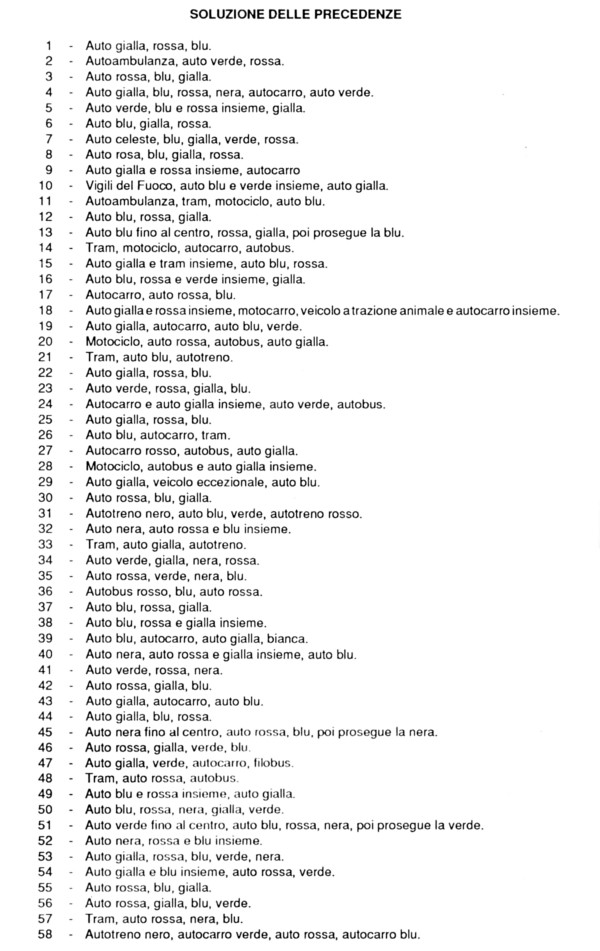
\includegraphics[width=1.25\textwidth]{images/sol}
	}
	\label{fig:sol}
\end{figure}

\restoregeometry

Prestando attenzione, si nota che gli incroci, la cui soluzione è discordante da quella fornita dal sistema, sono il n. 15 e il n. 26:
\begin{figure}[htbp!]
	\centering
	\begin{subfigure}[b]{.4\textwidth}
		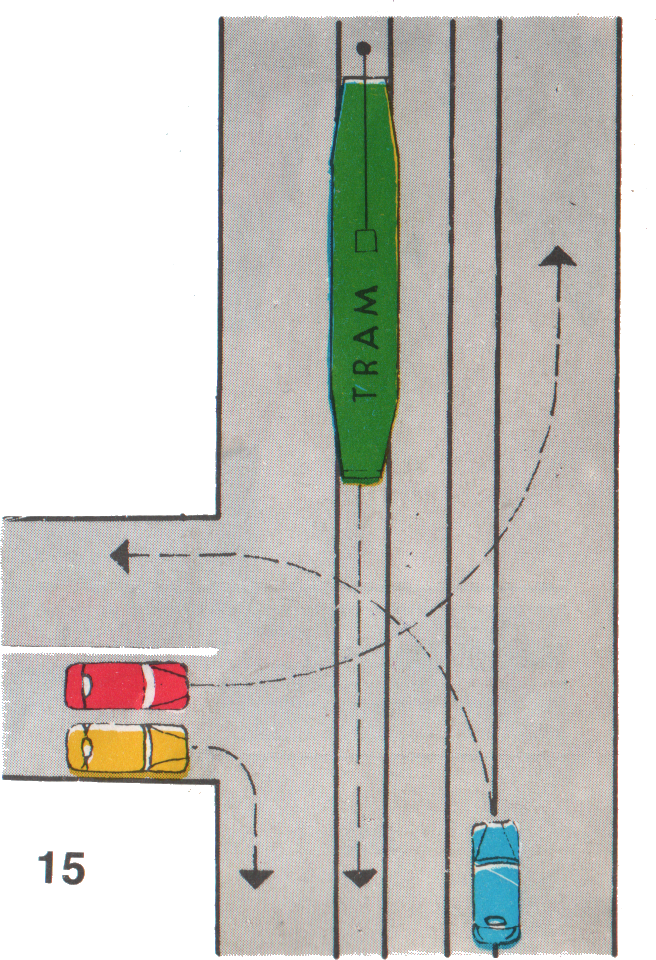
\includegraphics[width=\textwidth]{./images/fig15}
		\caption{Incrocio 15}
		\label{fig:15}
	\end{subfigure}
	\begin{subfigure}[b]{.4\textwidth}
		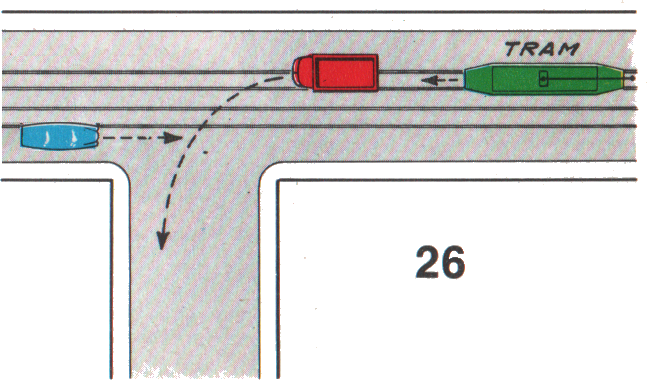
\includegraphics[width=\textwidth]{./images/fig26}
		\caption{Incrocio 26}
		\label{fig:26}
	\end{subfigure}
	\caption{Casi non conformi}
	\label{fig:disc}
\end{figure}



\begin{center}
	\begin{tabularx}{\textwidth}{cXXX}
		\hline
		\textbf{Incrocio} & \multicolumn{1}{c}{\textbf{Sistema}} & \multicolumn{1}{c}{\textbf{Prontuario}} & \multicolumn{1}{c}{\textbf{Spiegazione}} \\ \hline
		\adjustbox{raise=-1.4cm}{15} & 	\textit{Il veicolo tram è il primo a passare; 
					I veicoli blu, giallo passano insieme;
					Il veicolo rosso è l'ultimo a passare;} & \textit{Auto gialla e tram insieme, auto blu, rossa} & Il tram è prioritario, quindi passa per primo rispetto agli altri. Bisogna trattare il concetto di corsia, o di rotaie su strada.  \\ \hline
		\adjustbox{raise=-1.3cm}{26} & 	\textit{Il veicolo tram è il primo a passare;
				Il veicolo blu è il prossimo a passare;
				Il veicolo rosso è l'ultimo a passare;} & \textit{Auto blu, autocarro, tram} & Stesso motivo, il tram è prioritario. Bisogna trattare il concetto di coda tra veicoli. \\ \hline
	\end{tabularx}
\end{center}

\clearpage
\chapter{Conclusioni}

Il progetto ha proposto un risolutore di incroci, ritrovabili sugli esami della patente di guida e su eserciziari correlati. È stato definito un formalismo logico che spiegasse tutti gli oggetti coinvolti (veicoli, bracci, segnali ecc.), trasferendo poi la conoscenza in un software Prolog, arricchito anche da una componente grafica con l'ausilio del Java.

I risultati sono soddisfacenti: solo 2 incroci su 58 non risultano conformi alle regole, quindi in futuro sarà necessario espandere e modificarle per coprire anche questi casi.

Un domani si potrebbe anche realizzare un modulo di riconoscimento e caricamento di un incrocio partendo direttamente dalle immagini, senza dover trascrivere i fatti a mano, che può risultare tedioso.
\clearpage
\clearpage
\bibliographystyle{abbrvnat}
\bibliography{mybib}

\newpage

\end{document}